% XCircuit output "rfTransmitter-raw.tex" for LaTeX input from rfTransmitter-raw.ps
\def\putbox#1#2#3#4{\makebox[0in][l]{\makebox[#1][l]{}\raisebox{\baselineskip}[0in][0in]{\raisebox{#2}[0in][0in]{\scalebox{#3}{#4}}}}}
\def\rightbox#1{\makebox[0in][r]{#1}}
\def\centbox#1{\makebox[0in]{#1}}
\def\topbox#1{\raisebox{-0.60\baselineskip}[0in][0in]{#1}}
\def\midbox#1{\raisebox{-0.20\baselineskip}[0in][0in]{#1}}
   \scalebox{1}{
   \normalsize
   \parbox{11.7604in}{
   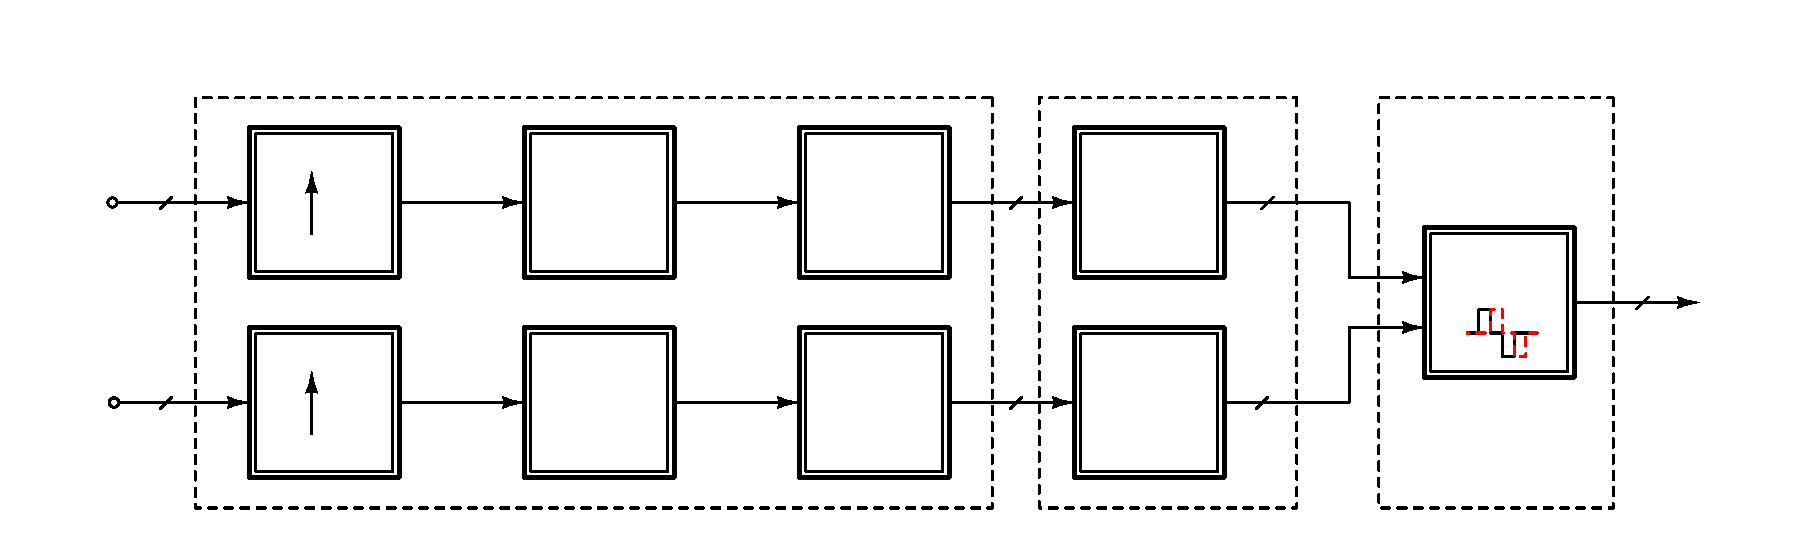
\includegraphics[scale=1]{rfTransmitter-raw}\\
   % translate x=1055 y=327 scale 0.38
   \putbox{2.05in}{0.68in}{2}{$8$}%
   \putbox{0.07in}{2.09in}{1.80}{$I[n]$}%
   \putbox{0.06in}{0.76in}{1.80}{$Q[n]$}%
   \putbox{3.72in}{2.01in}{2}{$z^{-\frac{T}{8}}$}%
   \putbox{3.72in}{0.68in}{2}{$z^{\frac{T}{8}}$}%
   \putbox{5.43in}{2.17in}{2}{$\Delta/\Sigma$}%
   \putbox{5.39in}{0.83in}{2}{$\Delta/\Sigma$}%
   \putbox{7.24in}{2.17in}{2}{$\mathrm{LUT}$}%
   \putbox{9.56in}{1.54in}{2}{$\mathrm{RFIQ}$}%
   \putbox{7.25in}{0.84in}{2}{$\mathrm{LUT}$}%
   \putbox{5.57in}{1.85in}{1.20}{4-bit}%
   \putbox{5.57in}{0.52in}{1.20}{4-bit}%
   \putbox{2.05in}{2.00in}{1.20}{$8$}%
   \putbox{10.76in}{1.23in}{1}{1-bit}%
   \putbox{11.27in}{1.38in}{1.80}{$y[n]$}%
   \putbox{1.19in}{3.14in}{1.80}{\textbf{Podsistem I}}%
   \putbox{6.82in}{3.14in}{1.80}{\textbf{Podsistem II}}%
   \putbox{9.08in}{3.14in}{1.80}{\textbf{Podsistem III}}%
   \putbox{1.19in}{2.90in}{1.60}{$f_s \to 8f_s$}%
   \putbox{6.82in}{2.91in}{1.60}{$8f_s \to 8Mf_s$}%
   \putbox{9.08in}{2.95in}{1.60}{$8Mf_s \to 4\cdot 8 Mf_s$}%
   \putbox{7.36in}{0.52in}{1.20}{M-bit}%
   \putbox{7.36in}{1.85in}{1.20}{M-bit}%
   \putbox{0.84in}{1.89in}{1}{N-bit}%
   \putbox{0.84in}{0.56in}{1}{N-bit}%
   \putbox{6.51in}{1.89in}{1}{4-bit}%
   \putbox{6.50in}{0.57in}{1}{4-bit}%
   \putbox{8.22in}{1.89in}{1}{1-bit}%
   \putbox{8.22in}{0.56in}{1}{1-bit}%
   } % close 'parbox'
   } % close 'scalebox'
   \vspace{-\baselineskip} % this is not necessary, but looks better
